In this note, we describe the phenomenology of dark matter models involving a strong coupling to the top quark.
These models can be classified according to their experimental signatures. Assuming the Standard Model (SM) flavour scheme, 
the models essentially lead to $\ttbar + \met$ final state and are described in a separated document. Since we do not know the flavour structure
of the dark sector, it is also interesting to relax this constraint and consider a different experimental signatures: monotop final state ($t+\met$)
and a prompt production of two top quarks having the same electric charge ($tt$)\footnote{For simplicity, the notation $tt$ is used to describe both $tt$ 
and $\bar{t}\bar{t}$}. These two final states are forbidden at the leading order in the SM
and become thus a good area to search for any new physics, and in particular dark matter.

\subsection{Model structure}

As usual, a dark matter candidate $\chi$ and a mediator $M$ (vectorial or scalar) need to be added to the SM to describe the dark sector and its
interaction with the SM particles. The full details of the various models are described in~\cite{AndreaFuksMaltoni,Agram:2013wda,,Cacciapagliaetal}, the basic ingredients are the following:
\begin{enumerate}
 \item the theory is effective and respects the $\SUtwoUone$ symmetry,
 \item the mediator strongly couples to the top quark,
 \item the top quark is \textit{singly} produced in association with a new particle $\Xnew$ (dark matter or mediator).
\end{enumerate}

There are two classes of models based on the monotop production mode: resonant and non-resonant production, as shown
in Fig.~\ref{fig:feyn_prod}. The sections~\ref{sec:ResonantProd} and~\ref{sec:NonResonantProd} describe the phenomenology leading to such production mechanisms.
Depending on the nature of $\Xnew$, two main final states might be relevant: monotop production or same-sign top quark pair production. 
Section~\ref{sec:ColliderSignature} discusses how the interplay of these two signatures can largely probe this class of dark matter model.

\begin{figure}[!h!tpd]
\centering
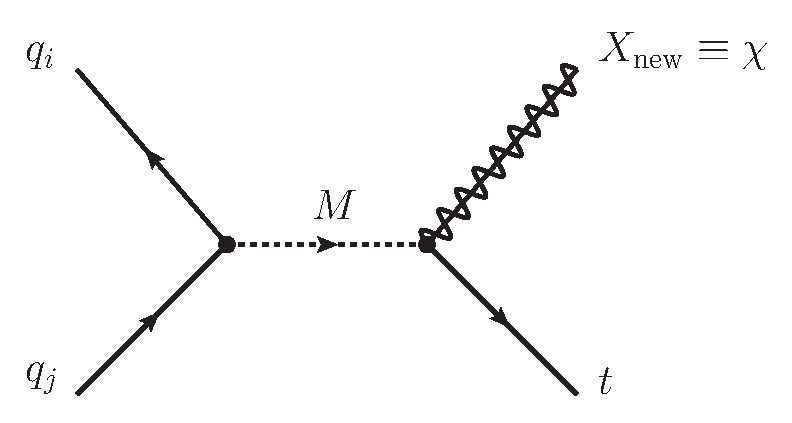
\includegraphics[width=0.31\textwidth]{feyn_diags/Resonant}
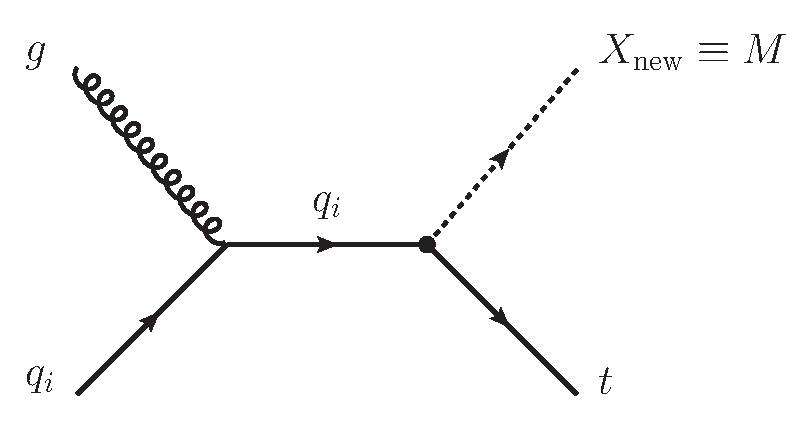
\includegraphics[width=0.31\textwidth]{feyn_diags/NonResonant}
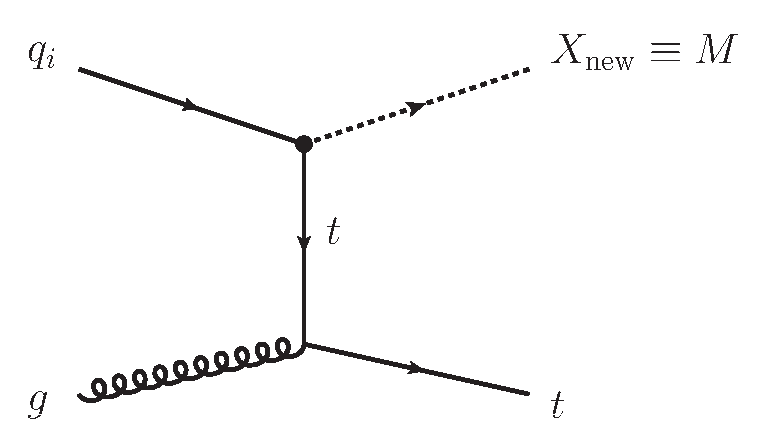
\includegraphics[width=0.31\textwidth]{feyn_diags/NonResonant2}
%\subfigure[\label{subfig:S1}]{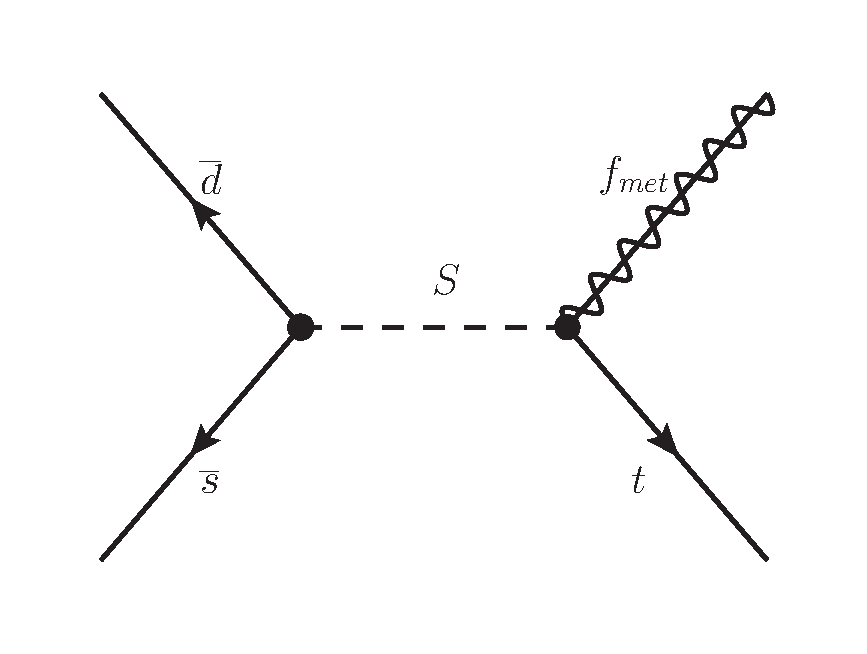
\includegraphics[width=0.46\textwidth]{feyn_diags/S1}}\\
%\subfigure[\label{subfig:S4_s}]{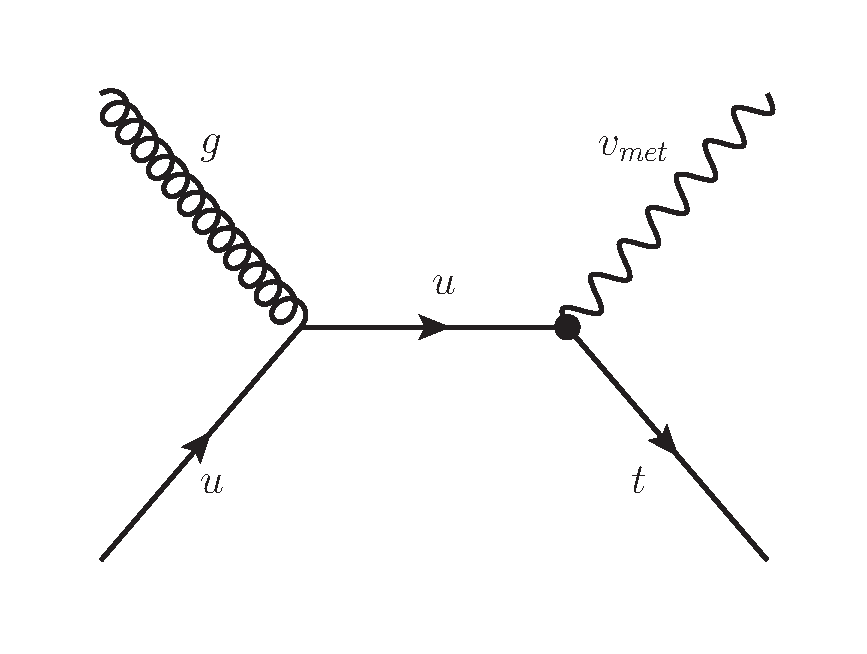
\includegraphics[width=0.46\textwidth]{feyn_diags/S4_s}}
%\subfigure[\label{subfig:S4_t}]{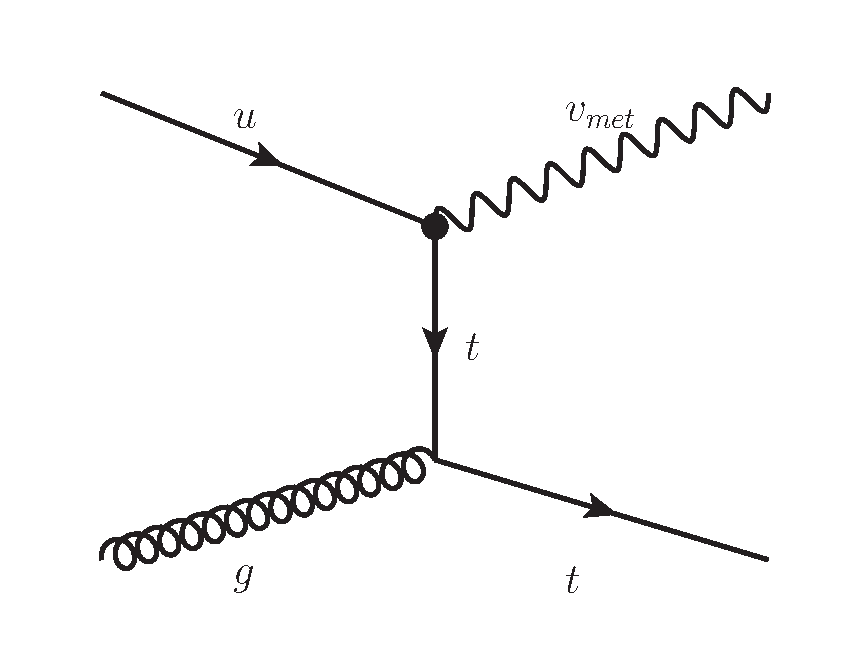
\includegraphics[width=0.46\textwidth]{feyn_diags/S4_t}}
\caption
{
%Feynman diagram of leading order processes leading to monotop events: production of
%a coloured scalar resonance $S$ decaying into a top quark and a spin-$1/2$ fermion $f_{met}$
%in the $\mathrm{S1_R}$ model~\subref{subfig:S1}, and $s$-\subref{subfig:S4_s}
%and $t$-\subref{subfig:S4_t} channel non resonant production of a top quark in association with
%a spin-1 boson $v_{met}$ in the $\mathrm{S4_R}$ model.
Feynman diagram of leading order processes leading to monotop events: resonant production of
$t$ via resonant mediator $M$ decaying into a top quark and $\Xnew$, which is the dark matter fermion $\chi$ (left),
and $s$ and $t$ channel non-resonant production of a top quark in association with $\Xnew$, which is the mediator $M$ (middle and right).
}
\label{fig:feyn_prod}

\end{figure}


\subsubsection{Resonant production}
\label{sec:ResonantProd}

In this case, the mediator $M$ is a couloured $2/3$-charged scalar $\phi^{\pm}$ decaying into a top quark and a spin-$1/2$ invisible particle, $\chi$ 
($\Xnew$ is then the dark matter candidate $\chi$). The dynamics of the new sector is then described by the following lagrangian:
\begin{equation}
 \label{eq:lagrangianResonant}
 \Lagr_{\mathrm{int}} \; = \; d^{C}_{i} \:  \left[ \left(g^{v}_{\phi d}\right)^{ij} +  \left(g^{a}_{\phi d}\right)^{ij} \gam^{5} \right] \: d_{j} \: \phi^{\pm} \; 
 + \; u^{C}_{k}  \left[ \left(g^{v}_{u\chi}\right)^{k} + \left(g^{a}_{u\chi}\right)^{k} \gam^{5} \right] \: \chi \: \phi^{\pm}
\end{equation}
where $u$ ($d$) stands for any $up$-quark ($down$-quark), the index $v$ ($a$) stands for vectorial (axial), $C$ means charge conjugate and $i,j,k$ run over the generations (color 
indices involved in the $\phi^{\pm}-$quarks interaction are not explicitly written).
The first term leads to the production of the mediator and the last term allows its decay into a $up$-quark 
and a non interacting fermion (in particular to the top quark when $\left(g^{v/a}_{u\chi}\right)^{k}$ is sizable mainly for $k=3$).
This model is then described by the masses of the mediator $m_{\phi}$ and the invisible fermion $m_{\chi}$, and the coupling 
$\left(g^{v/a}_{\phi d}\right)^{ij}$ and $\left(g^{v/a}_{u\chi}\right)^{k}$.

\com{Question/comment: in this resonant model, this is not so obvious to interpret $\phi_{\pm}$ as the mediator since there is a vertex $\phi-u-\chi$.
It is somehow breaking the concept of having a dark sector weakly coupled to ordinary matter via a mediator.}


\subsubsection{Non-resonant production}
\label{sec:NonResonantProd}

For the non-resonant production, the top quark is produced in association with the mediator 
($\Xnew$ is then the mediator and not the dark matter candidate). They are two possibilities 
depending on the nature of the mediator.

First, the mediator can be a scalar field interacting with the SM field and the dark matter candidate as described in this lagrangian:
\begin{equation}
 \label{eq:lagrangianNonResonantScalar}
 \Lagr_{\mathrm{int}} \; = \; u^{C}_{i} \:  \left[ \left(g^{v}_{\phi u}\right)^{ij} +  \left(g^{a}_{\phi u}\right)^{ij}  \gam^{5} \right] \: u_{j} \: \phi \; 
 + \; \chi^{C}  \left[ g^{v}_{\phi\chi} + g^{a}_{\phi\chi}  \gam^{5} \right] \chi \: \phi
\end{equation}
where $u$ stands for any $up$-quark, the index $v$ ($a$) stands for vectorial (axial), $C$ means charge conjugate and $i,j,k$ run over the generations.
The first term describes the interaction between the mediator and the $up$-quarks while the second term leads to the decay the mediator 
into invisible fermions. In this model, there is necessarily a mixing between $\phi$ and  the Higgs boson field. Additional parameters 
are then required to describe this new sector. Indeed, on top of the mediator mass and couplings, the mixing matrix of the two scalar fields
is needed in order to make predictions. For the sake of simplicity, we do not consider this case were the parameters 
space would be too large.

Another possibility is to consider a vectorial field as mediator with the following dynamics:
\begin{equation}
 \label{eq:lagrangianNonResonantVector}
  \Lagr_{\mathrm{int}} \; = \; \bar{u}_{i} \left[ \left(g^{v}_{Vu}\right)^{ij} \gam^{\mu} + \left(g^{a}_{Vu}\right)^{ij} \gam^{5} \right] u_{j} \: V_{\mu} \; 
  + \; \bar{\chi} \left[ g^{v}_{Vu} \gam^{\mu} + g^{a}_{V\chi} \gam^{5} \right]   \chi \: V_{\mu}
\end{equation}
where $u$ stands for any $up$-quark, the index $v$ ($a$) stands for vectorial (axial) and $i,j,k$ run over the generations.
The first term describes the interaction between the mediator and the $up$-quarks while the second term leads to the decay the mediator 
into invisible fermions. The new sector can be defined with the couplings $\left(g^{v/a}_{Vu}\right)^{ij}$, 
$g^{a/v}_{V\chi}$ and the masses $m_V$ and $m_{\chi}$. This model can be probed by two experimental signatures 
depending on the exact scenario: monotop and same-sign top quark production. 

\com{Question for theorists: why it cannot mix with $\Zboson$ in case of vectorial mediator ?}

